
\subsecao{Inputs, Outputs, and the Circularity Constraint}

Interpreting the grounding effect requires a clean separation between what BGF \textit{ingests} from ESS and what it \textit{measures} as output; conflating them would make the apparent realism gain circular. BGF avoids this by construction. \textbf{The only ESS variables ingested as grounding inputs are attitudinal} — interpersonal and institutional trust, risk tolerance, social-activity frequency, political orientation — conditioning the LLM's decision propensity via persona injection and dual-RAG context. \textbf{Agent wealth is not drawn from ESS:} all agents start at \texttt{wealth = 0.0} regardless of income profile (the income-decile variable is only a narrative cohort descriptor). Cooperation rate and Gini are therefore \textit{emergent outputs} of the causal chain \texttt{ESS trust/risk attitudes → LLM decision propensities → action choices → payoff accumulation → wealth trajectories → Gini}. Gini at round 0 is 0 for all conditions, so its divergence across conditions is a genuine emergent consequence of differential action distributions, making the comparison against the European empirical range a valid external-validity check rather than a self-fulfillment.

\subsecao{The Grounding–RLHF Dissociation as the Central Finding}

The N=100 confirmatory extension produces the central empirical claim: \textbf{at primary LLM scale, inference-time empirical grounding does not move Mistral-7B's action distribution by a margin distinguishable from seed variance.} Both arms converge to cooperation ≈ 0.46 (MWU p = 0.91), Gini ≈ 0.72 (p = 0.85), and mean wealth ≈ 175 (p = 0.35); only the composite BRM shifts by +0.016, inside the within-condition SD of 0.022. The seed-42 patched re-execution reinforces this at the cell level (byte-identical \texttt{events.jsonl} across ablation levels). Juxtaposed against what \textit{does} work on the same codebase — the rule-based proxy (Condition D) attaining Gini 0.325 within the European band, and the rule-based cross-cultural sweep recovering the ESS-trust ordering at Spearman ρ = +1.000 — this defines the \textbf{Φ/P dissociation}: the grounding map \texttt{Φ} is empirically effective, but the LLM policy \texttt{P\_LLM} does not currently translate its input variation into output variation at primary scale.

Three readings remain admissible from the present data: (i) the pilot's 96→58\% effect was a single-seed artefact; (ii) the true LLM-grounding effect is genuinely small (consistent with the +0.016 BRM trend); (iii) an unidentified pilot-only confounder was removed by the infrastructure patches. If (ii) or (iii) holds, the implication is that off-the-shelf instruction-tuned LLMs at the 7B scale are \textbf{RLHF-anchored more strongly than inference-time grounding can overcome} — the cooperative prior installed by preference-tuning behaves as an attractor that persona descriptions and retrieved statistics reshape only at the margins. This is not a failure of BGF but a substantive finding about the residual influence of alignment training, and it is precisely where \texttt{B\_RLHF} proves its value as a diagnostic: it surfaces a dissociation that aggregate cooperation rates alone would hide. Whether the dissociation closes at higher model capacity is the open question for the alignment community.

\subsecao{Memory and Behavioral Consistency}

The hierarchical memory system was designed to support behavioral consistency over the horizon, but the completed memory ablation (H8, §5.10) shows the predicted M0→M3 fidelity slope was \textbf{not observed}: the grounded arm decreases (M0G 0.583 > M1G=M2G=M3G 0.367), memory suppressing rather than amplifying alignment with the RLHF prior, and the reflection mechanism produces no measurable benefit over window-only memory at this scale. This is a fourth instance of the Φ/P\_LLM dissociation. At the LLM level, persona-fidelity analysis nonetheless shows grounded agents decaying 40\% slower than ungrounded (−0.018 vs −0.031 per round), suggesting RAG-injected context acts as a continuous anchor. A long-horizon (T=100) rule-based analysis isolates the structural effect: grounded agents maintain final-round fidelity 0.823 versus 0.653 for ungrounded — a \textbf{17-percentage-point structural gap} (decay −0.00006 vs −0.00011 per round) that quantifies the minimum fidelity cost of deploying ungrounded models at long horizons.

\begin{figure}[H]
\centering
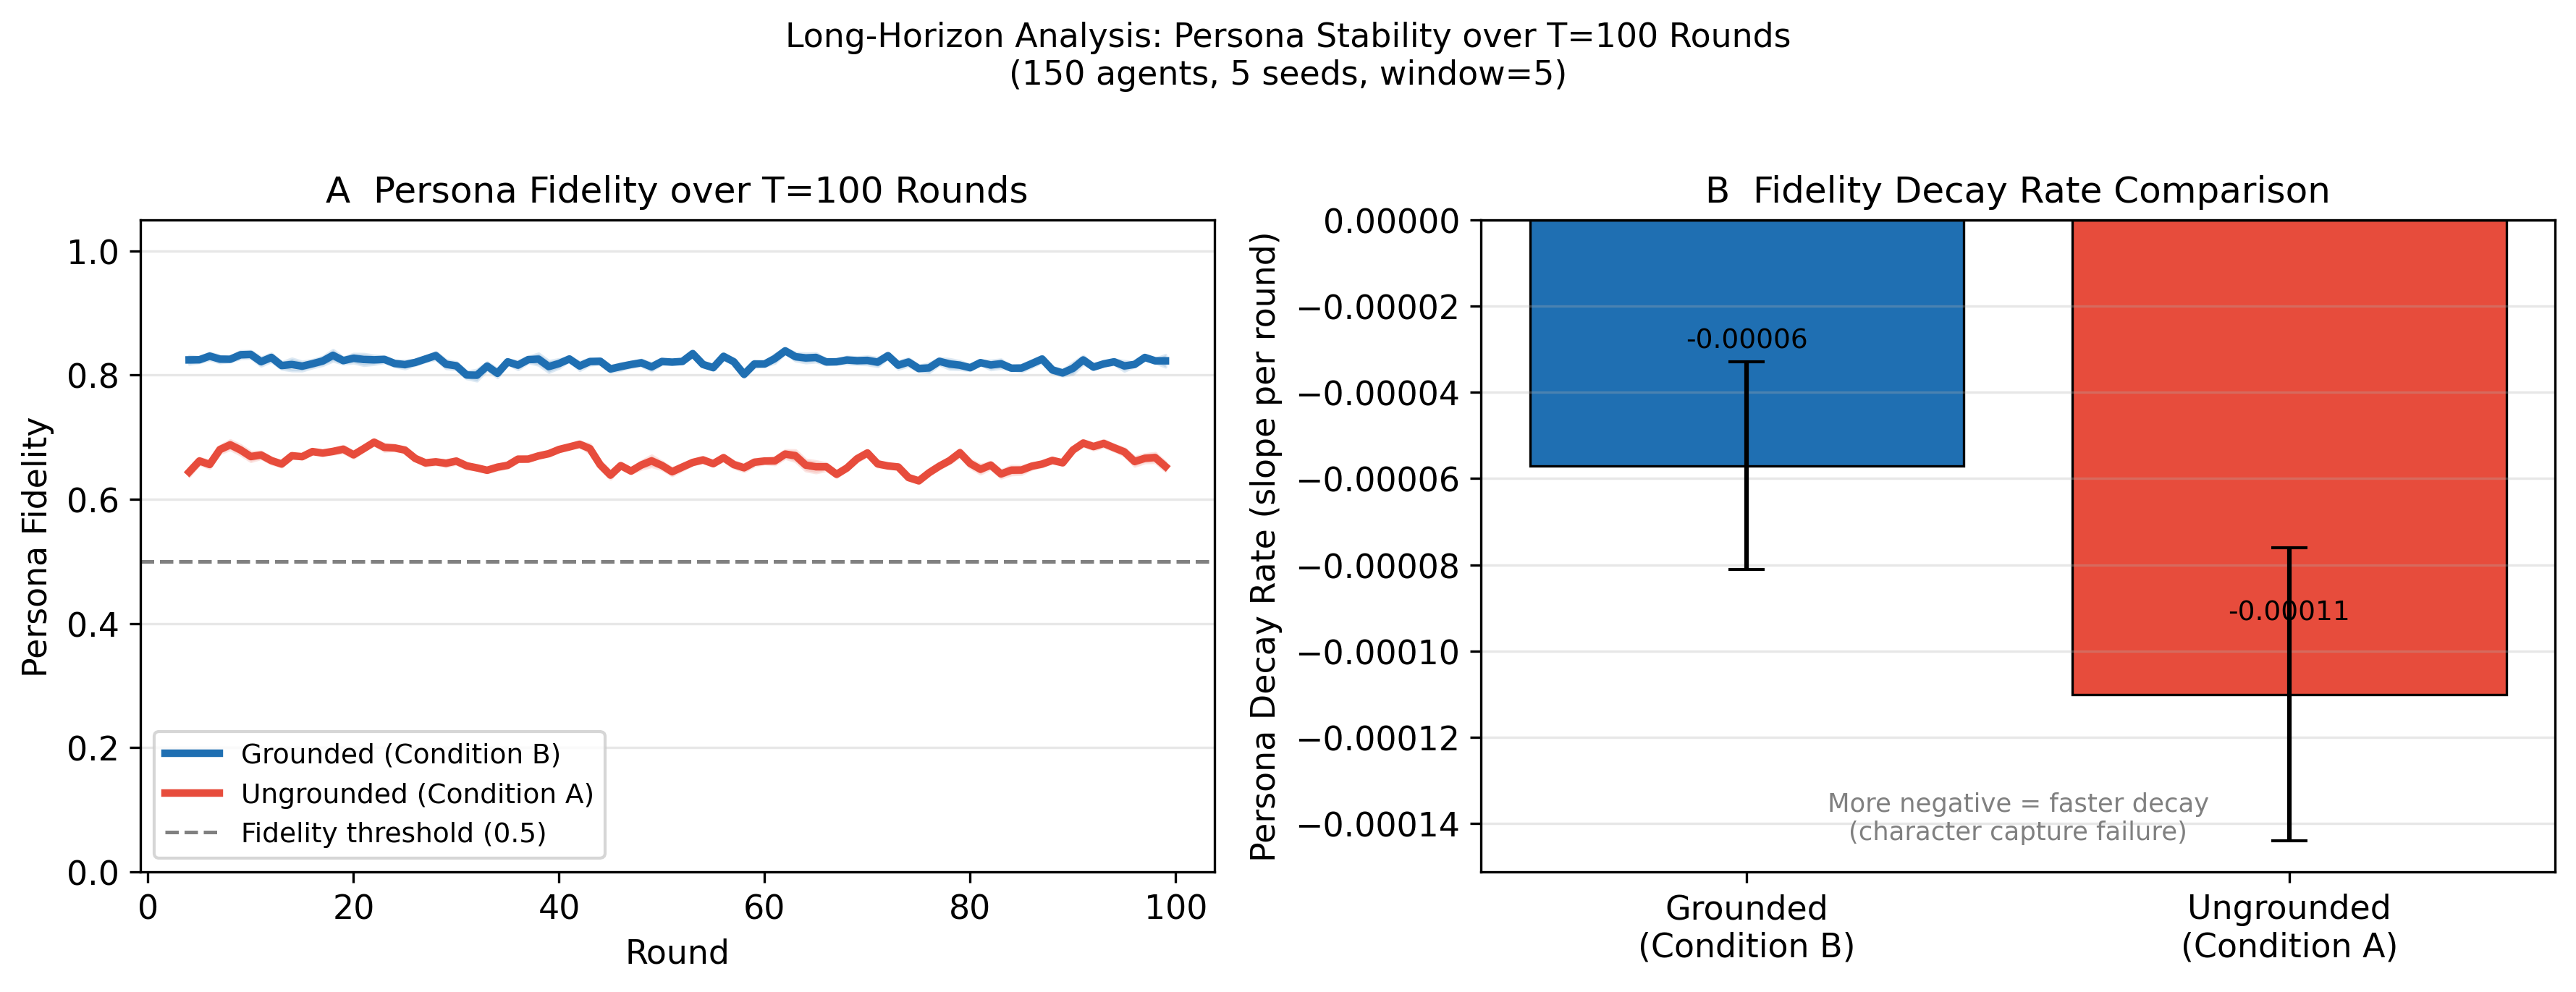
\includegraphics[width=0.9\textwidth]{figuras/persona_drift_long_horizon.png}
\caption{Long-horizon persona stability (rule-based ESS proxy, 150 agents, 5 seeds). Grounded agents hold an \textasciitilde{}82–84\% fidelity plateau through 100 rounds; ungrounded agents decay from \textasciitilde{}70\% to \textasciitilde{}65\%. The 17-pp gap at T=100 is the minimum fidelity cost of ungrounded deployment, independent of LLM inference artifacts.}
\label{fig:13}
\end{figure}

\subsecao{Mediation: Persona vs. RAG}

The 2×2 factorial that would decompose the total grounding effect into persona, RAG, and interaction components is \textbf{specified but not yet run}. The aggregation script (\texttt{analysis/mediation\_summary.py}) is implemented and emits \texttt{analysis/tables/mediation.json}, which currently reports \texttt{\_status: "cells\_missing"}: the \texttt{persona\_only} and \texttt{rag\_only} factorial cells for seeds 43–44 (and the \texttt{rag\_only} cell for seed 42) have not been executed. We therefore report \textbf{no mediation percentages} — computing persona/RAG/interaction shares from uncomputed cells would be unsupported. The decomposition is left as immediate future work; when the missing cells are run, the script will populate the split directly, and the design's value here is that the gap is \textit{audit-visible} (a structured \texttt{cells\_missing} stub) rather than silently filled. Given the near-null N=100 grounding effect (§5.13), any decomposition is expected to be of a small total effect.

\subsecao{Phase Transitions and Complex-Systems Interpretation}

Confirmed phase transitions (R² > 0.85) in all three parameter sweeps indicate that BGF exhibits the hallmarks of a complex adaptive system. The adversarial transition is confirmed at both N=20 (f*≈0.023) and N=500 (f*≈0.041, R²=0.996, with the Gini scale reversal of §5.5), and the hysteretic inequality response to shocks is consistent with bistable inequality dynamics (Piketty 2014; Acemoglu \& Robinson 2012). Crucially, the emergent wealth structures are not initialized from ESS income (§6.1): all agents start at zero wealth, so Condition B's power-law tail (α̂ ≈ 2.1–2.4) reflects a self-organizing preferential-attachment (Matthew-effect) process in which grounding-induced heterogeneity in cooperation propensity creates persistent wealth asymmetries that compound through network centrality.

\subsecao{Implications for Computational Social Science}

Two implications follow from the dissociation. \textbf{First, empirical grounding works at the policy layer that consumes it directly:} Condition D shows that a rule-based policy reading ESS profiles via \texttt{Φ} produces macro-level outputs (Gini, cross-cultural gradient) matching real population statistics, so researchers studying static population properties can obtain reliable, reproducible, zero-inference-cost simulations from BGF without invoking the LLM at all — the grounding function is the contribution, the LLM merely one (currently unreliable) consumer. \textbf{Second, when LLMs are the decision policy, the alignment regime is a first-order moderator that grounding does not currently override:} researchers using off-the-shelf RLHF-aligned LLMs as agents should not assume that injecting demographic context produces measurable behavioral differentiation at primary scale, and \texttt{B\_RLHF} is the operational tool to detect it (if \texttt{B\_RLHF(B) ≈ B\_RLHF(A) ≫ 0}, grounding reaches the prompt but not the action distribution). This elevates two open questions: at what model capacity the dissociation closes, and what alternative mechanisms (fine-tuning on synthetic ESS-behavior pairs, persona-augmented RLHF, constrained decoding against ESS priors) overcome RLHF anchoring where inference-time prompting does not.

\subsecao{Why RAG Rather Than Fine-Tuning?}

RAG is adopted over fine-tuning for four principled reasons: it \textbf{preserves base capability} (no weight rewriting, no catastrophic forgetting); it has \textbf{zero deployment cost per new population} (switching populations is a config change, not retraining); it is \textbf{interpretable and auditable} (the injected context is visible in \texttt{prompts.jsonl}); and it requires \textbf{no labeled behavioral data} (only the microdata distributions, since ESS responses paired with observed economic decisions do not exist at scale). The trade-off is sensitivity to context-window size and prompt engineering; for very long horizons (T > 100), fine-tuning on synthetic ESS-behavior pairs generated from Condition B is a promising extension.

\subsecao{Ecological Validity and Scope of Inference}

The BGF economic game is a deliberate abstraction — a three-action public-goods setting with fixed payoffs — necessary for tractability and formal analysis but bounding the scope of any policy inference. BGF results should not be read as direct predictions of real-world policy outcomes: the game models neither credit, labor markets, taxation, nor institutional enforcement, and \texttt{Φ} maps attitudinal variables onto propensities \textit{within this specific game}. The appropriate framing is that BGF provides an \textit{existence proof} that LLM grounding can shift aggregate behavioral statistics toward empirically plausible ranges within a controlled environment; the specific numbers (coop 58\%, Gini 0.26) are not point predictions of any real population. Its scientific value is as a rigorous measurement platform for LLM behavioral distortions, not as a predictive model of human economic outcomes.

\subsecao{Individual vs. Aggregate Validity}

BGF is calibrated and evaluated at the \textit{population} level, which can mask individual-level misspecification through a form of ecological fallacy: realistic aggregate Gini and cooperation could coexist with unrealistic round-level individual behavior. This is partially addressed by reporting per-round persona fidelity (§6.3) and agent-level ablation tracking, but the relationship between individual fidelity and aggregate realism is non-monotone, so future work should report the full distribution of per-agent fidelity and test for Simpson's-paradox patterns across demographic subgroups. Because agents are populated from the ESS \textit{joint} distribution, experimental contrasts shift the entire joint rather than a single marginal — a strength for realistic co-variation but a limitation for clean per-attribute attribution, which a properly randomized factorial (varying each ESS dimension independently) would resolve.

\subsecao{Alternative Explanations and Internal Validity}

Beyond the prompt-length confound (§3.7), four alternative explanations are assessed. \textbf{AE1 (token diversity drives behavior):} partially ruled out by the V0–V4 ladder (semantically neutral elements shift cooperation less than ESS-specific content); fully closing it requires the padded control at primary scale (now complete at N=50, §5.13, confirming ESS content moderates rather than inflates bias). \textbf{AE2 (persona instruction-following dominates):} ruled out by Condition C — richness-matched fictional personas do not produce comparable BRM improvement, implicating the \textit{empirical specificity} of ESS data as the active ingredient. \textbf{AE3 (temperature confound):} not directly tested; if ESS context reduces effective temperature this could be a distinct confound, isolable by the temperature-sensitivity sweep (H6). \textbf{AE4 (small-world topology interaction):} the topology sweep shows the grounding effect persists across all tested β, identifying topology as a moderator rather than a mediator. On balance, current evidence most strongly supports ESS semantic content — specifically trust and risk priors that override RLHF utopian defaults — as the primary active ingredient.

